\documentclass[12pt,handout]{beamer}


\xdefinecolor{lavendar}{rgb}{0.8,0.6,1}
\xdefinecolor{olive}{cmyk}{0.64,0,0.95,0.4}
%\xdefinecolor{olive}{cmyk}{1,0,0,0}
\xdefinecolor{mag}{cmyk}{0.1,1,0,0.2}
\xdefinecolor{lblue}{rgb}{0,0,1.5}
\xdefinecolor{lred}{rgb}{1,0,0}
\xdefinecolor{mine}{cmyk}{1,0,0.2,0}
\xdefinecolor{bluel}{cmyk}{0.1,0,0.9,0.4}

\usepackage{amsmath,amssymb,dsfont,mathrsfs}
\usepackage{tikz,pgflibraryplotmarks}
\usepackage{multimedia}
\usepackage{wasysym}
\usepackage{rotating}
\usepackage{algorithm,algorithmic}
\usepackage{graphicx} % more modern
\usepackage{subfigure}
\usepackage{booktabs}

\usepackage{pgfplots}
\usepackage{verbatim}

\usepackage{setspace}
\newlength\iwidth
\newlength\iheight

\newcommand\makebeamertitle{\frame{\maketitle}}%
\graphicspath{{./images/}}
\setbeamertemplate{navigation symbols}{}
\addtobeamertemplate{navigation symbols}{}{%
    \usebeamerfont{footline}%
    \usebeamercolor[fg]{footline}%
	\insertshorttitle
    \;--
    \insertframenumber
}

\newcommand{\sectionstart}{
	\only<beamer>{
 	\begin{frame}% (fold)
 		\begin{centering}\Huge \insertsection \par\end{centering}
 	\end{frame}% frame the_application (end)
	}
 }


% make bibliography entries smaller
\usepackage{natbib}
\setbeamertemplate{bibliography item}{[\theenumiv]}
\renewcommand\bibfont{\scriptsize}
\setbeamertemplate{frametitle continuation}[from second]
\newcommand{\tcr}{\textcolor{red}}
\newcommand{\tcrd}{\textcolor{red}}
\newcommand{\tcb}{\textcolor{bluel}}
\newcommand{\tcm}{\textcolor{mag}}
\newcommand{\tcg}{\textcolor{olive}}

\newcommand{\R}{\mathbb{R}}
\newcommand{\C}{\mathbb{C}}

% bold lower-case for vectors
\newcommand{\bfa}{{\bf a}}
\newcommand{\bfb}{{\bf b}}
\newcommand{\bfc}{{\bf c}}
\newcommand{\bfs}{{\bf s}}
\newcommand{\bfm}{{\bf m}}
\newcommand{\bfd}{{\bf d}}
\newcommand{\bfe}{{\bf e}}
\newcommand{\bfu}{{\bf u}}
\newcommand{\bfy}{{\bf y}}
\newcommand{\bfx}{{\bf x}}
\newcommand{\bfh}{{\bf h}}
\newcommand{\bfw}{{\bf w}}
\newcommand{\bfv}{{\bf v}}
\newcommand{\bfr}{{\bf r}}
\newcommand{\bfz}{{\bf z}}
\newcommand{\bfp}{{\bf p}}


% bold upper-case for linear operators
\newcommand{\bfA}{{\bf A}}
\newcommand{\bfB}{{\bf B}}
\newcommand{\bfZ}{{\bf Z}}
\newcommand{\bfM}{{\bf M}}
\newcommand{\bfC}{{\bf C}}
\newcommand{\bfD}{{\bf D}}
\newcommand{\bfQ}{{\bf Q}}
\newcommand{\bfJ}{{\bf J}}
\newcommand{\bfG}{{\bf G}}
\newcommand{\bfI}{{\bf I}}
\newcommand{\bfP}{{\bf P}}
\newcommand{\bfK}{{\bf K}}
\newcommand{\bfY}{{\bf Y}}
\newcommand{\bfW}{{\bf W}}
\newcommand{\bfR}{{\bf R}}
\newcommand{\bfL}{{\bf L}}
\newcommand{\bfF}{{\bf F}}
\newcommand{\bfT}{{\bf T}}
\newcommand{\bfS}{{\bf S}}
\newcommand{\bfX}{{\bf X}}
\newcommand{\bfU}{{\bf U}}
\newcommand{\bfV}{{\bf V}}
\newcommand{\bfH}{{\bf H}}


\newcommand{\calF}{\mathcal{F}}



\newcommand{\hf}{{\frac 12}}
\newcommand{\bftheta}{{\boldsymbol \theta}}
\newcommand{\bfxi}{{\boldsymbol \xi}}

\newcommand{\bfLambda}{{\boldsymbol \Lambda}}
\newcommand{\bfSigma}{{\boldsymbol \Sigma}}
\newcommand{\bfepsilon}{{\boldsymbol \epsilon}}

\newcommand{\E}{\vec E}
\newcommand{\B}{\vec B}

\newcommand{\vu}{  {\vec {\bf u}}}

\newcommand{\grad}{  {\vec {\bf \nabla}}}

\newcommand{\lfrownie}{\textcolor{red}{\large{\frownie}}}
\newcommand{\lsmiley}{\textcolor{green}{\large{\smiley}}}

\newcommand{\curl}{\ensuremath{\nabla\times\,}}
\renewcommand{\div}{\nabla\cdot\,}
\newcommand{\divh}{\nabla_h\cdot\,}
\renewcommand{\grad}{\ensuremath{\nabla}}

\DeclareMathOperator*{\argmin}{arg\,min}

\title{Spectral Clustering for Unsupervised Learning}
\subtitle{Numerical Methods for Deep Learning}
\date{}


\begin{document}
\makebeamertitle


%% ------------------------------------------------------------
%% ------------------------------------------------------------
%% ------------------------------------------------------------

\section{Motivation} % (fold)
\label{sec:motivation}
\begin{frame}
\frametitle{Motivation: Data Mining}


Assume we have data 
  
$$\bfY = [\bfy_1, \ldots, \bfy_n]$$.

The data can be
\begin{itemize}
\item Images
\item Text
\item Sound
\item Set of numbers (climate, pressure ...)
\end{itemize}

\bigskip

We can think of (at least) three goals:
\begin{itemize}
\item Cluster the data (unsupervised)
\item Give meaning to each cluster, label it (semisupervised)
\item Find a functional relation between the cluster and its label (supervised)
\end{itemize}

\end{frame}

\begin{frame}
\frametitle{Example: Un/Semi/Fully Supervised Learning}


Example: $\bfy \in \R^2$ contains rock conductivity porosity

\begin{center}
	\begin{tabular}{ccc}
		unsupervised & semi-supervised \\
		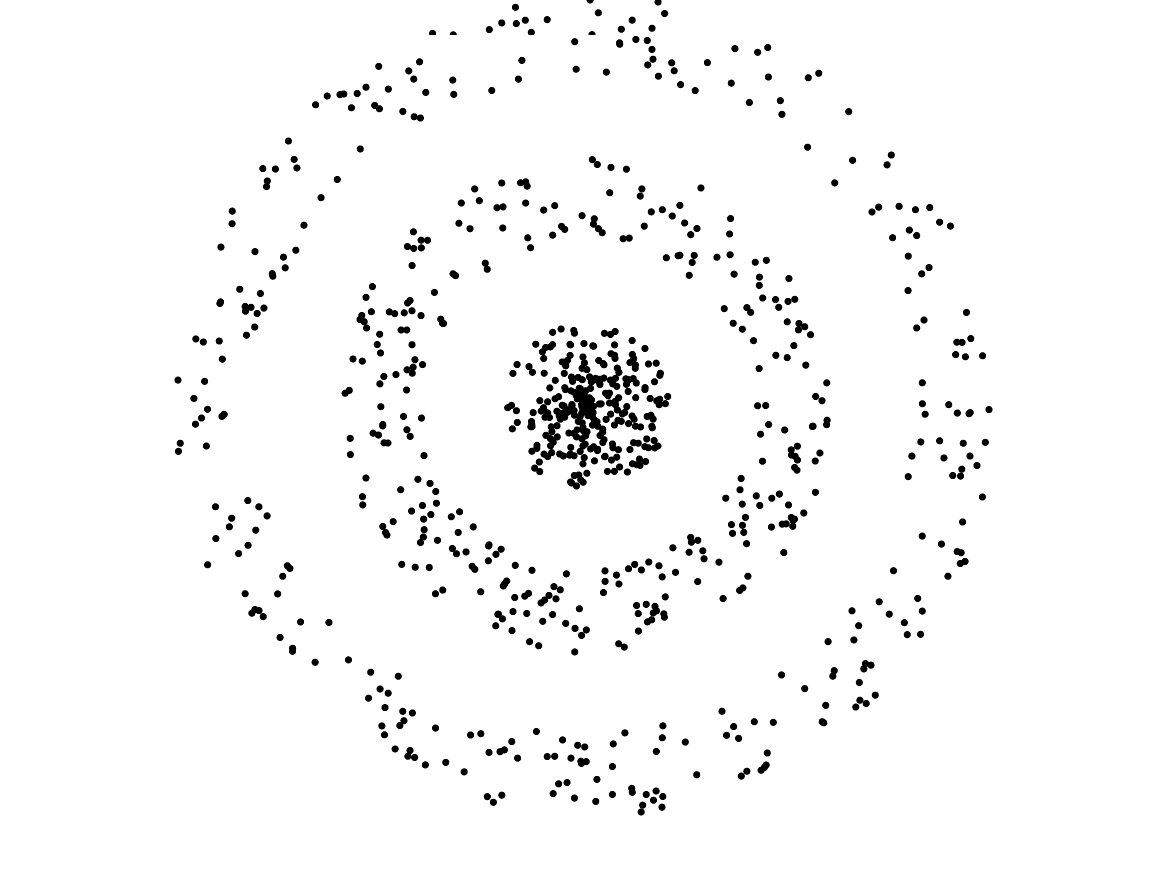
\includegraphics[width=0.4\textwidth]{unsupervised_data}&
		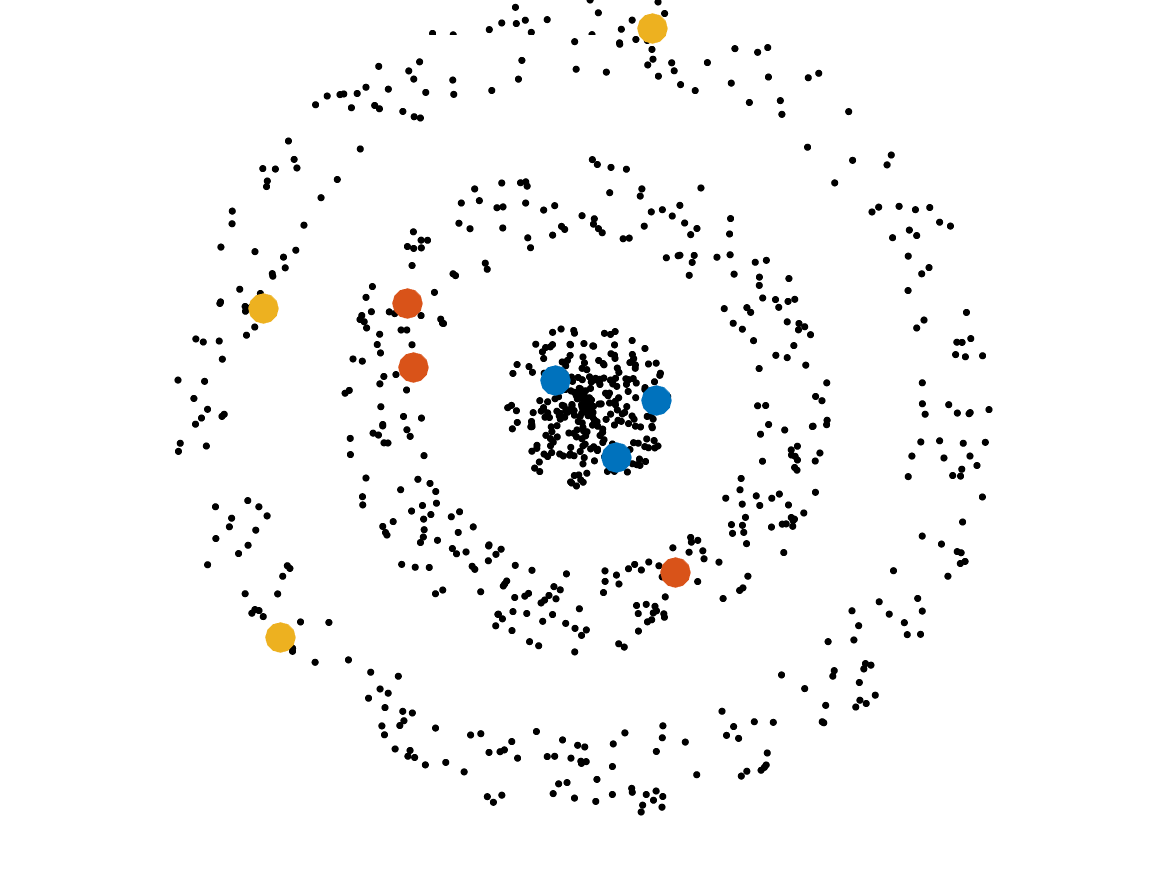
\includegraphics[width=0.4\textwidth]{unsupervised_semi}		
	\end{tabular}
\end{center}

\begin{itemize}
\item How many types of rocks do we have? {\bf Unsupervised learning}
\item What are their names (Granite, Basalt)? {\bf Semisupervised learning}
\item Given $\sigma, \phi$ can we find a function $f(\sigma,\phi) = {\rm rock\ type}$? {\bf Supervised learning}
\end{itemize}


\end{frame}

\begin{frame}
\frametitle{Discussion: Un/Semi/Fully Supervised Learning}


\begin{itemize}
\item Supervised learning requires a large labeled data set
\item Gives an "explanation" (a model) between data and label
\item Un/Semisupervised is more modest
\item No model, just label
\item Can be followed by supervised learning
\end{itemize}


\end{frame}


\begin{frame}
\frametitle{Learning Objective: Spectral Clustering}

In this module we focus on spectral clustering algorithms for unsupervised and semisupervised learning.

\bigskip

Learning tasks:
\begin{itemize}
\item Given a data set cluster the data into a few groups
\item Assuming that a few data are labeled, label the rest
\end{itemize}

\bigskip

Numerical methods:
\begin{itemize}
	\item k-means algorithm (not discussed)
	\item spectral clustering (our focus)
\end{itemize}

\end{frame}
\begin{frame}
\frametitle{Spectral Clustering: General Idea}

{\bf Idea:}
Given the data set $\bfY = [\bfy_1, \ldots, \bfy_n]$, if $\bfy_i$ is similar to
$\bfy_j$ then they belong to the same class.

\bigskip

Central question: How to measure and use similarity?

\begin{center}
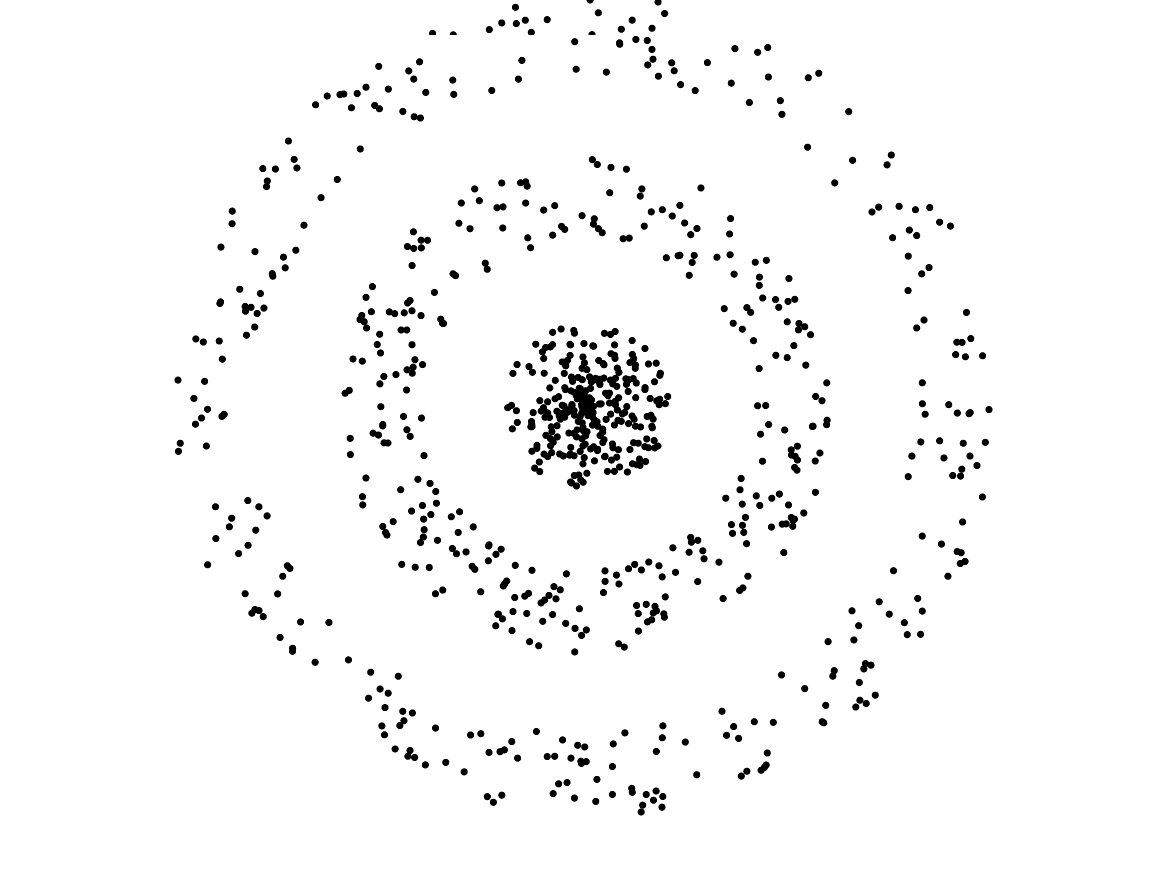
\includegraphics[width=5cm]{unsupervised_data.png}	
\end{center}

Literature: \cite{NgEtAl2002,PothenEtAl1990,vonLuxburg2007}
\end{frame}

% section motivation (end)


\section{Similarity Measures} % (fold)
\label{sec:section_name}

\begin{frame}
\frametitle{Similarity Measures: Metrics - 1}

How to quantify the similarity of two data points?

\bigskip

A function $D : \R^{n_f} \times \R^{n_f} \rightarrow [0,\infty)$ is called a \emph{metric}, if for all $\bfx,\bfy,\bfz$ it holds that
\begin{itemize}
\item  $D(\bfx,\bfy) \ge 0$
\item $D(\bfx,\bfy) = 0 \quad \Rightarrow \quad \bfx = \bfy$
\item $D(\bfx,\bfy) = D(\bfy,\bfx)$
\item $D(\bfx,\bfz) \le D(\bfx,\bfy) + D(\bfy,\bfz)$
\end{itemize}	

\bigskip

A metric can be used to measure similarity.

\bigskip

Note: Not all properties are needed. E.g., sometimes we will drop the second one.

\end{frame}

\begin{frame}
\frametitle{Similarity Measures: Metrics - 2}

Most obvious metric is induced by a norm, e.g.,
$$ D(\bfx,\bfy) = \|\bfx - \bfy\|_p = \left( \sum_{i=1}^{n_f} |\bfx_i-\bfy_i|^p \right)^{\frac 1p} $$

\begin{itemize}
\item most used is the $2$-norm (why?)
\item $p=\infty$ is called the max norm (why?)
\end{itemize}

\bigskip

A simple modification: weighted norms
$$ D(\bfx,\bfy) = \left( \sum_{i=1}^{n_f} \bfw_i |\bfx_i-\bfy_i|^p \right)^{\frac 1p} $$
where $\bfw >0$ is a vector of positive weights.
Allows us to focus on some components and scale the metric.
\end{frame}

\begin{frame}
\frametitle{Similarity Measures: Metrics - 3}

Are these signals similar?

\begin{center}
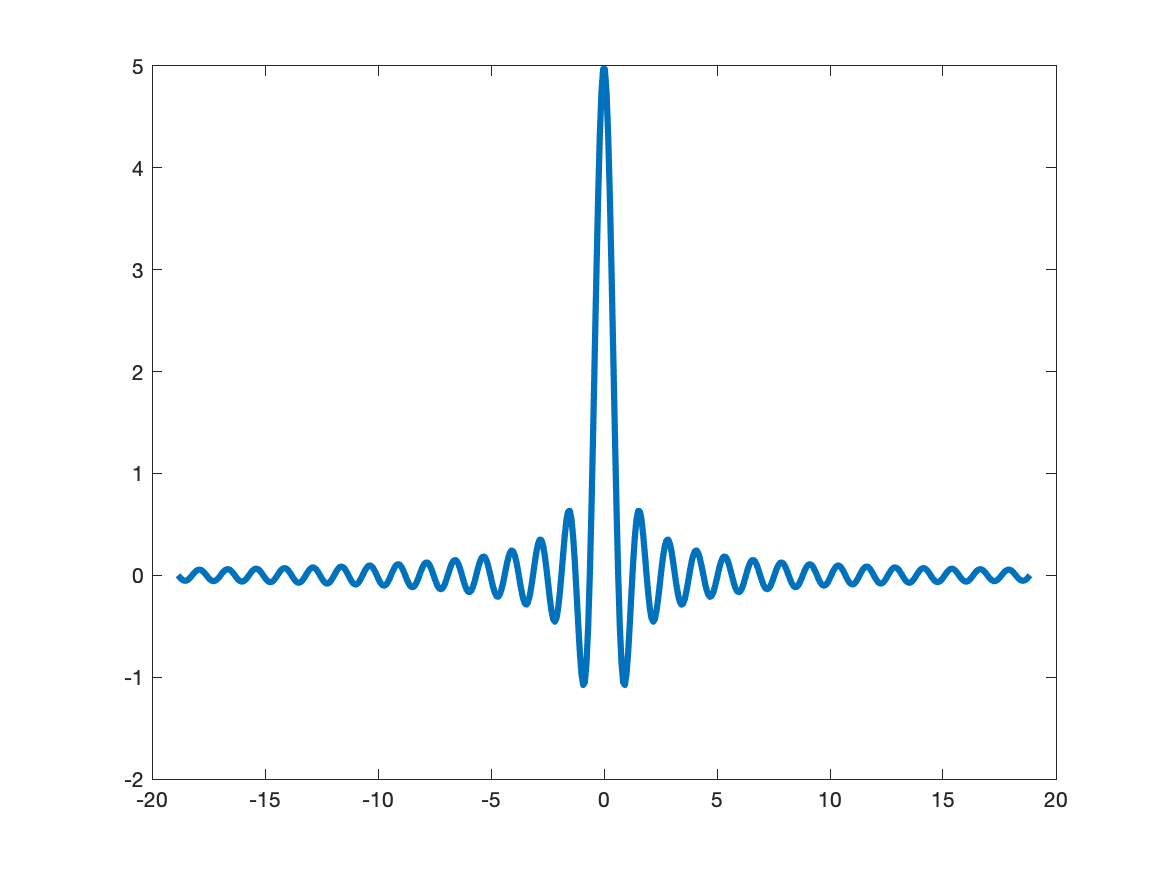
\includegraphics[width=5cm]{sincSignal1.png}
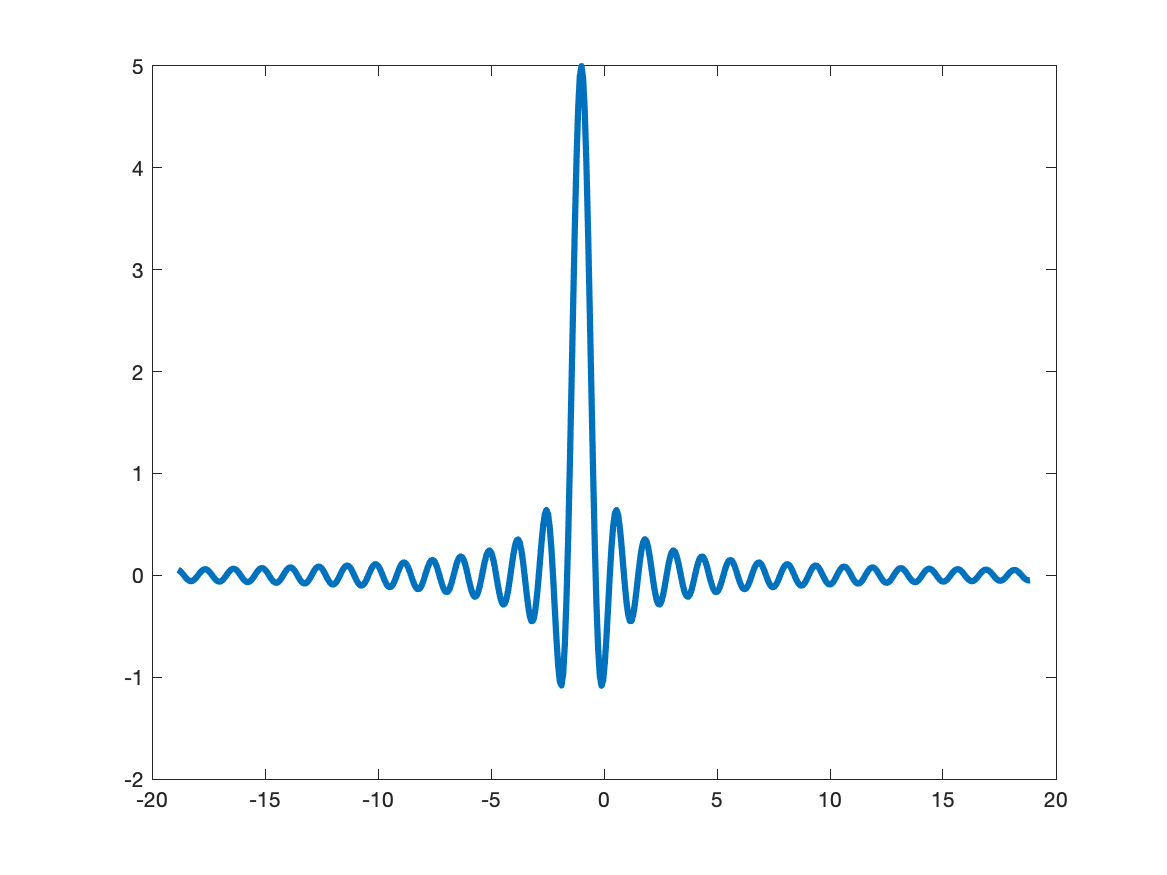
\includegraphics[width=5cm]{sincSignal2.png}
\end{center}

Can we find a translation-invariant metric?

\end{frame}

\begin{frame}
\frametitle{Similarity Measures: Metrics - 4}

Which of these image pairs are most similar?

\begin{center}
	\begin{tabular}{@{}c@{ }c@{ }c@{}}
		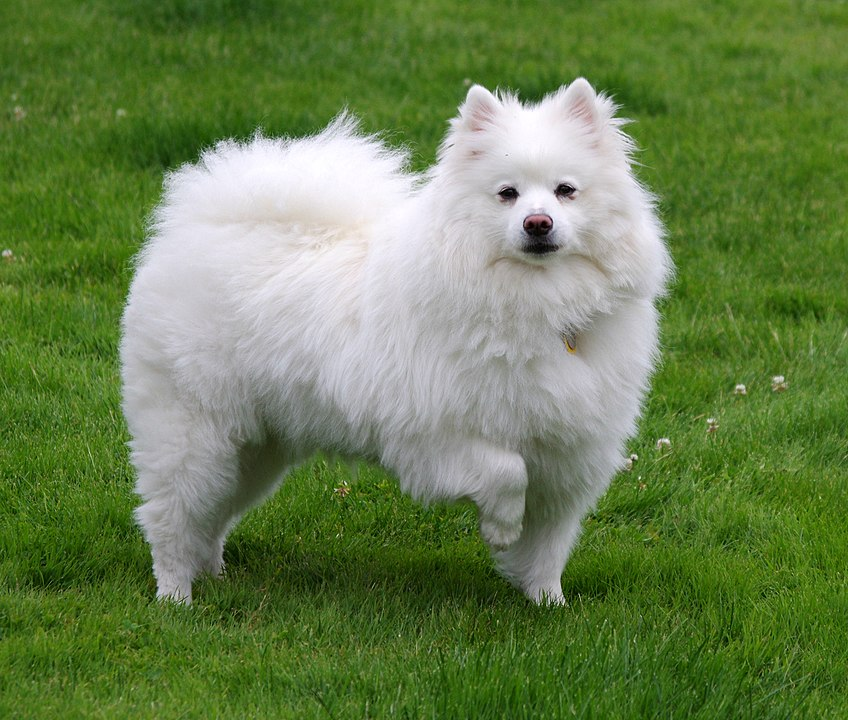
\includegraphics[height=2.5cm]{whiteDogCC} &
		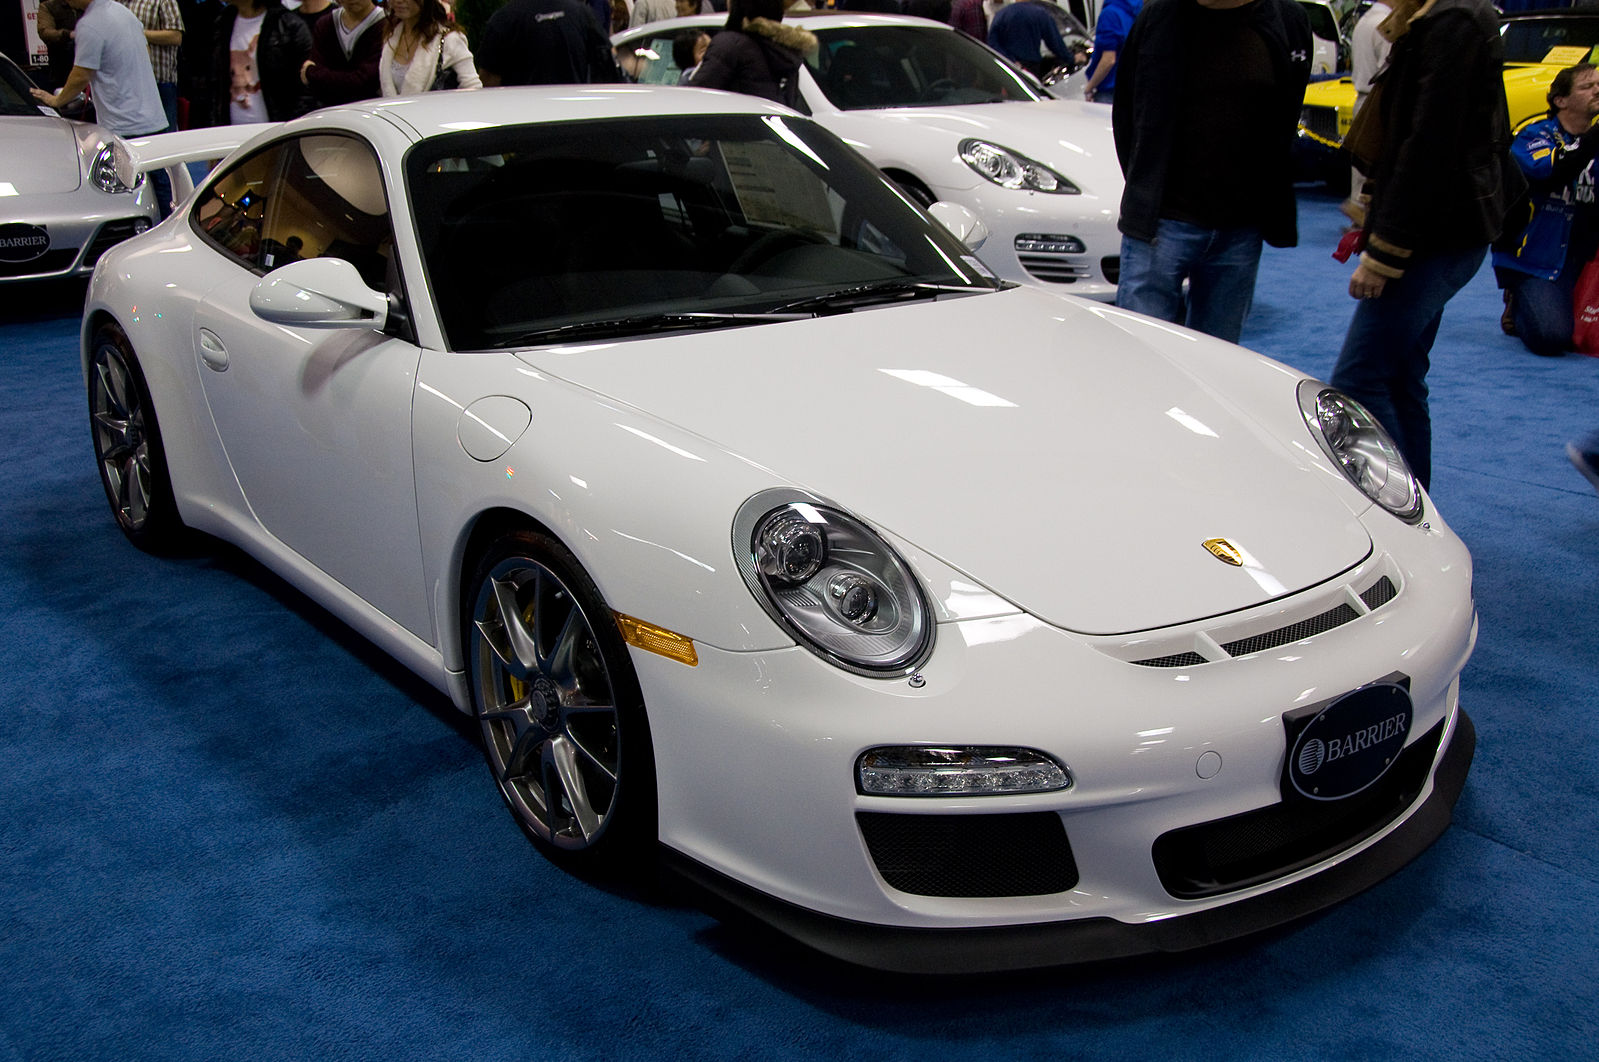
\includegraphics[height=2.5cm]{whiteCarCC}& 
		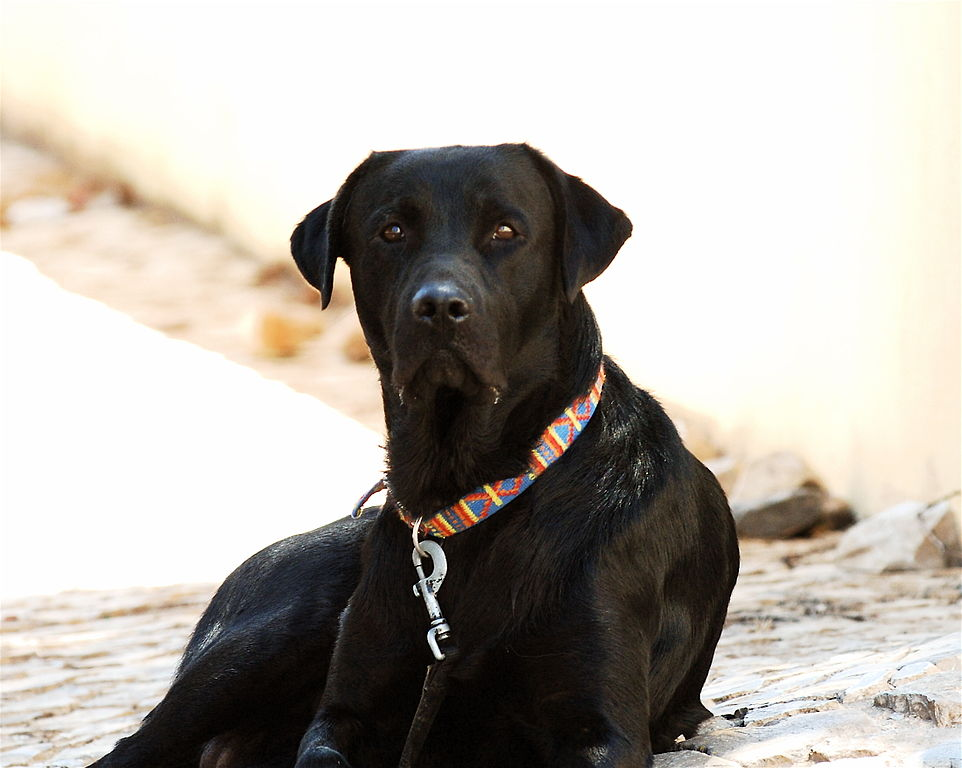
\includegraphics[height=2.5cm]{blackDogCC}\\
		\scriptsize \href{https://commons.wikimedia.org/w/index.php?curid=20509768}{(by Christmas w/a K)} &
		\scriptsize \href{https://commons.wikimedia.org/w/index.php?curid=12225485}{(by Art Bromage)} &
		\scriptsize \href{https://commons.wikimedia.org/w/index.php?curid=38049555}{(by  P R Simões)} 
 % all images under CC BY-SA 2.0
 	\end{tabular}

\end{center}

\end{frame}

\begin{frame}
\frametitle{Similarity Measures: Metrics - 5}

Many different definitions of distance based on the application
\begin{itemize}
\item normed distance
\item Hamming distance - for strings
\item Wasserstein metric - for probabilities (also applied to images)
\item Riemannian metrics - for data that "lives" on manifolds
\end{itemize}

\bigskip

Choosing the right similarity measure is the key for the application.

In many cases - chicken and egg. If we know the right distance then we know how to cluster.

\bigskip

We will use $\|\cdot\|_2$ for simplicity.

\end{frame}

\section{Similarity Graphs} % (fold)
\label{sec:graph_models}
\begin{frame}[fragile]
\frametitle{Undirected Graphs}

The graph $G(\bfY,\cal E)$ is described by its vertices $\bfy_1, \ldots, \bfy_{n}$ and an edge set $\cal E$.

\bigskip

Example: 
\begin{columns}
	\column{.6\textwidth}
\begin{verbatim}
Y = [-1 0 .1 .5 -1.5; -1 1 0 0 1];
E = [1 2;1 2;2 3;1 3;3 4;2 4;2 5];
\end{verbatim}
	\column{.4\textwidth}
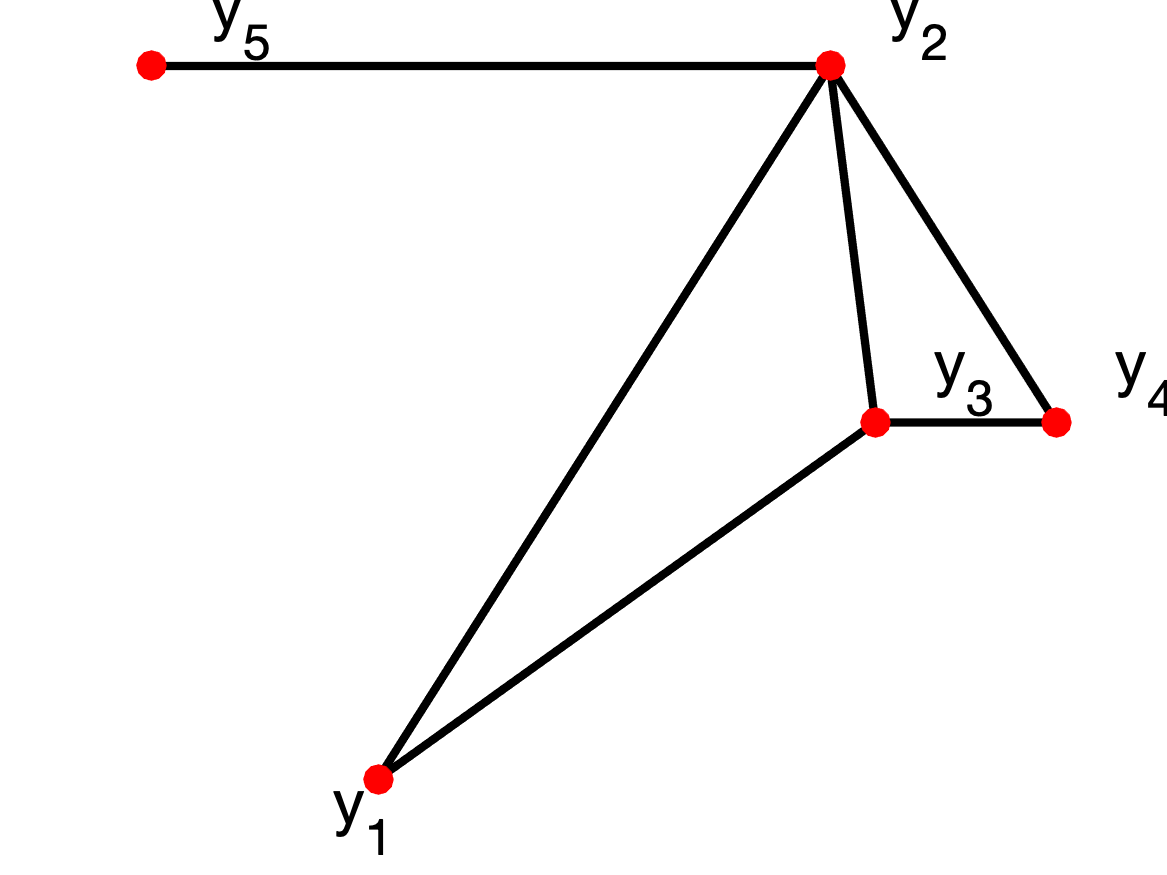
\includegraphics[width=4.5cm]{plotSimpleGraph}
\end{columns}

\bigskip


We will only use undirected graphs:  $(i,j) \in {\cal E} \Rightarrow (j,i) \in {\cal E}.$

\end{frame}


\begin{frame}
\frametitle{Adjacency Matrix of a Graph}

The adjacency matrix of $G(\bfY,\cal E)$ is  $\bfA \in \{0,1\}^{n \times n}$ with
\begin{equation*}
\bfA_{ij} = 	\begin{cases}
	 1, & \text{if  there is an  edge between $\bfy_i$ and $\bfy_j$} \\
	 0, & \text{else}.
	 \end{cases}
\end{equation*}

\begin{columns}
	\column{.5\textwidth}
	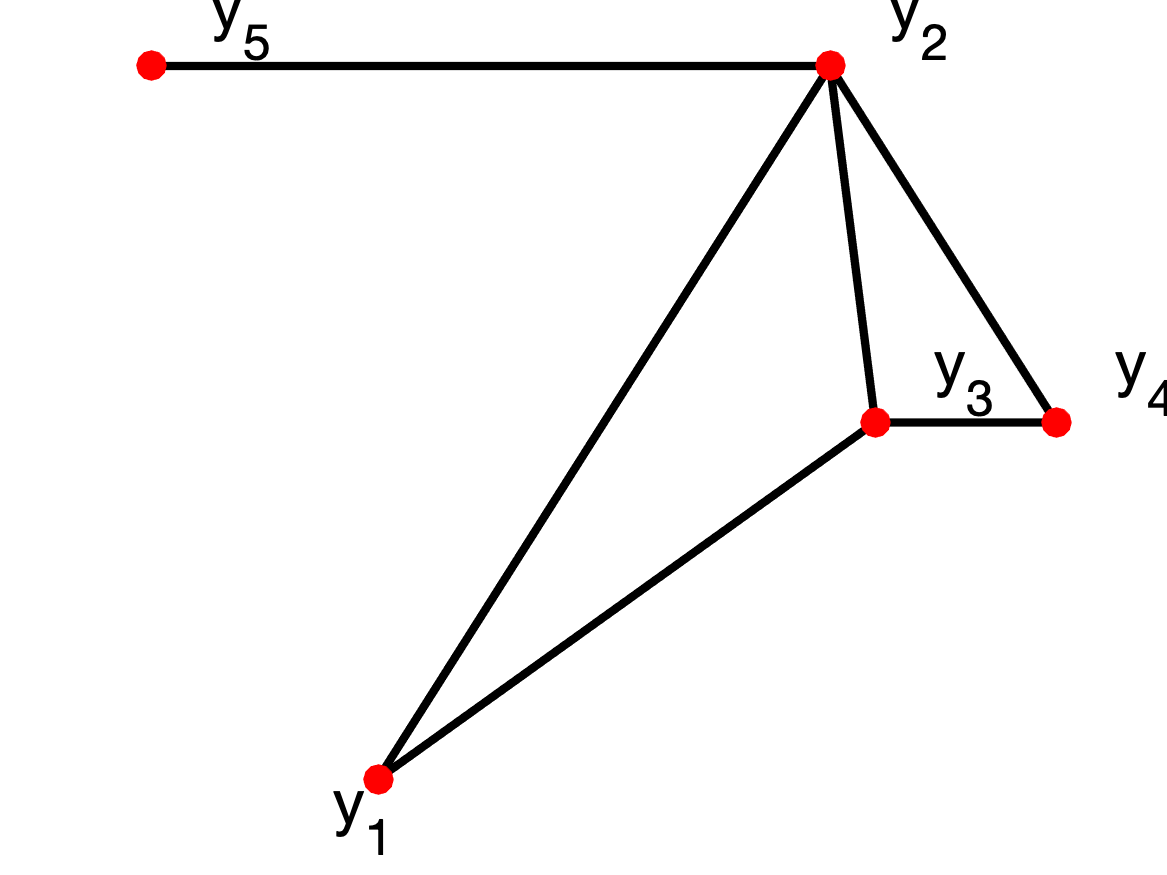
\includegraphics[width=4.5cm]{plotSimpleGraph}
	
	\column{.5\textwidth}
	$ \Rightarrow \bfA = \begin{pmatrix} 0 & 1 & 1 & 0 & 0 \\
	                         1 & 0 & 1 & 1 & 1 \\
	                         1 & 1 & 0 & 1 & 0 \\
	                         0 & 1 & 1 & 0 & 0 \\
	                         0 & 1 & 0 & 0 & 0 \end{pmatrix} $
\end{columns}

\begin{center}
Note: $\bfY$ and $\bfA$ fully describe the graph (no need to store $\cal E$).	
\end{center}
\end{frame}

\begin{frame}
\frametitle{Degree Matrix of a Graph}

The degree matrix is
$$ {\bfD}_{ii}   = {\rm diag}\left( \sum_j \bfA_{ij} \right)   \in \R^{n\times n}$$.

\bigskip

\begin{columns}
	\column{.5\textwidth}
	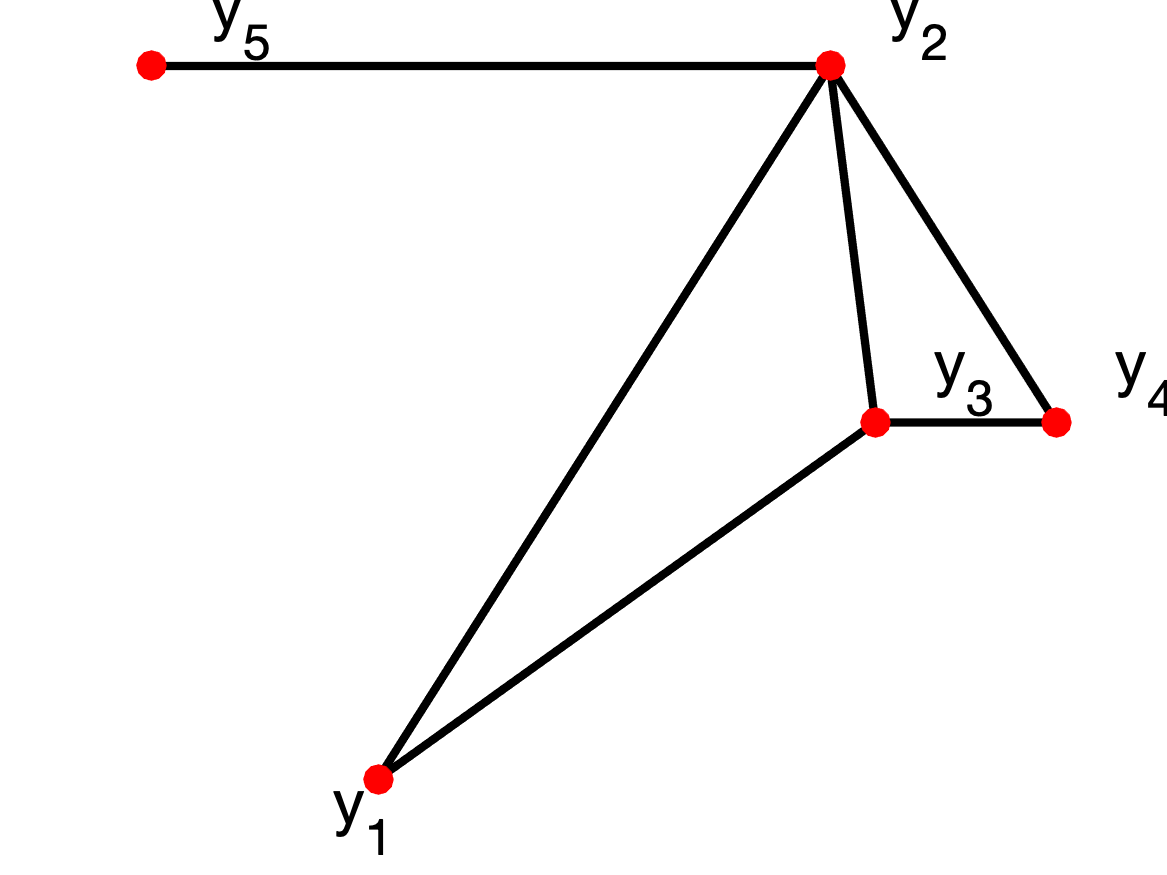
\includegraphics[width=4.5cm]{plotSimpleGraph}
	
	\column{.5\textwidth}
	$ \Rightarrow \bfD = \begin{pmatrix} 2 & 0 & 0 & 0 & 0 \\
	                                     0 & 4 & 0 & 0 & 0 \\
	                                     0 & 0 & 4 & 0 & 0 \\
	                                     0 & 0 & 0 & 2 & 0 \\
	                                     0 & 0 & 0 & 0 & 1 \end{pmatrix} $
\end{columns}

\bigskip

$\bfD_{ii}$ is the degree of node $\bfy_i$ ($\approx$ importance of $\bfy_i$). 

\end{frame}

\begin{frame}
\frametitle{Weighted Adjacency Matrix of a Graph}

The weighted adjacency matrix of $G(\bfY,\cal E)$ is  $\bfW \in \R_{+}^{n \times n}$ with
\begin{equation*}
\bfW_{ij}  \begin{cases}
		 > 0 & \text{ if } \bfA_{ij} = 1 \\
		 = 0 & \text{ otherwise.} 
\end{cases}	
\end{equation*}
Use a similarity measure to compute the entries in $\bfW$, e.g.,
$$ \bfW_{ij} = \exp\left(-{\frac {D(\bfy_i,\bfy_j)}{\sigma}} \right). $$

As before, the degree matrix is
$$ {\bfD}_{ii}   = {\rm diag}\left( \sum_j \bfW_{ij} \right)   \in \R^{n\times n}.$$


$\bfD_{ii}$ is the degree of node $\bfy_i$ ($\approx$ importance of $\bfy_i$). 

\end{frame}

\begin{frame}
	\frametitle{$k$-Nearest Neighbor Graph}
	Given: Data $\bfY$, $k \in \mathbb{N}$, and a distance function $D$.
	
	Idea: Set  $\bfA_{ij} = \bfA_{ji}=1$ if 
		$\bfy_i$ is among the $k$ nearest neighbors of $\bfy_j$ with respect to $D$ or vice versa.
		

    \bigskip
	
	This is not the only option. Common alternatives:
	\begin{itemize}
		\item \textbf{$\epsilon$-neighborhood graph: } add an edge between $\bfy_i$ and $\bfy_j$ if $D(\bfy_i,\bfy_j) < \epsilon$
		\item \textbf{mutual $k$-nearest neighborhood graph: } add an edge between $\bfy_i$ and $\bfy_j$ if 
		$\bfy_i$ is among the $k$ nearest neighbors of $\bfy_j$ \emph{and} vice versa.
		 \item \textbf{fully-connected graph: } add an edge between all examples. 
	\end{itemize}
	
	\bigskip
	
	In all these cases, we return the weighted adjacency matrix, whose entries depend on $D$.
	

\end{frame}

\section{Graph Laplacians} % (fold)
\label{sec:graph_laplacians}

\begin{frame}
\frametitle{The Graph Laplacian }

The graph Laplacian of $G(\bfY,{\cal E})$ is
$$ \bfL = \bfD  - \bfA $$ 

 For our example, we get

$$ \bfL = \left(\begin{array}{rrrrr} 2  & -1 & -1 & 0  & 0  \\
           				 -1 & 4  & -1 & -1 & -1 \\
           				 -1 & -1 & 4  & -1 & 0 \\
           				 0  & -1 & -1 & 2  & 0  \\
           				 0  & -1 & 0 & 0  & 1  \end{array} \right)$$

Note that for a vertex function $\bfv \in \R^n$
$$ (\bfL \bfv)_i =  \sum_{j=1}^n \bfA_{ij} (\bfv_i - \bfv_j) \quad \text{and} \quad \bfv^{\top}\bfL \bfv =  \sum_{i,j=1}^n  \bfA_{ij}(\bfv_i - \bfv_j)^2$$


\end{frame}

\begin{frame}
\frametitle{Weighted Graph Laplacian }

Similar to the previous slide, we define the weighted graph Laplacian of $G(\bfY,{\cal E})$ as
$$ \bfL = \bfD  - \bfW$$ 
($\bfD$ is the degree matrix of the weighted adjacency matrix $\bfW$)

\bigskip

For a vertex function $\bfv \in \R^n$, we obtain
$$ (\bfL \bfv)_i =  \sum_{j=1}^n \bfW_{ij} (\bfv_i - \bfv_j) \quad \text{and} \quad \bfv^{\top}\bfL \bfv =  \sum_{i,j=1}^n  \bfW_{ij}(\bfv_i - \bfv_j)^2$$

% In our experiments, we use
% $$ \bfW_{ij} = \exp\left(-{\frac {\|\bfy_i - \bfy_j\|^2}{\sigma}} \right) $$


\end{frame}

\begin{frame}
\frametitle{Eigenvalues of the Graph Laplacian}
\begin{center}
	\iwidth=32mm
\begin{tabular}{@{}c@{}c@{}c@{}}
	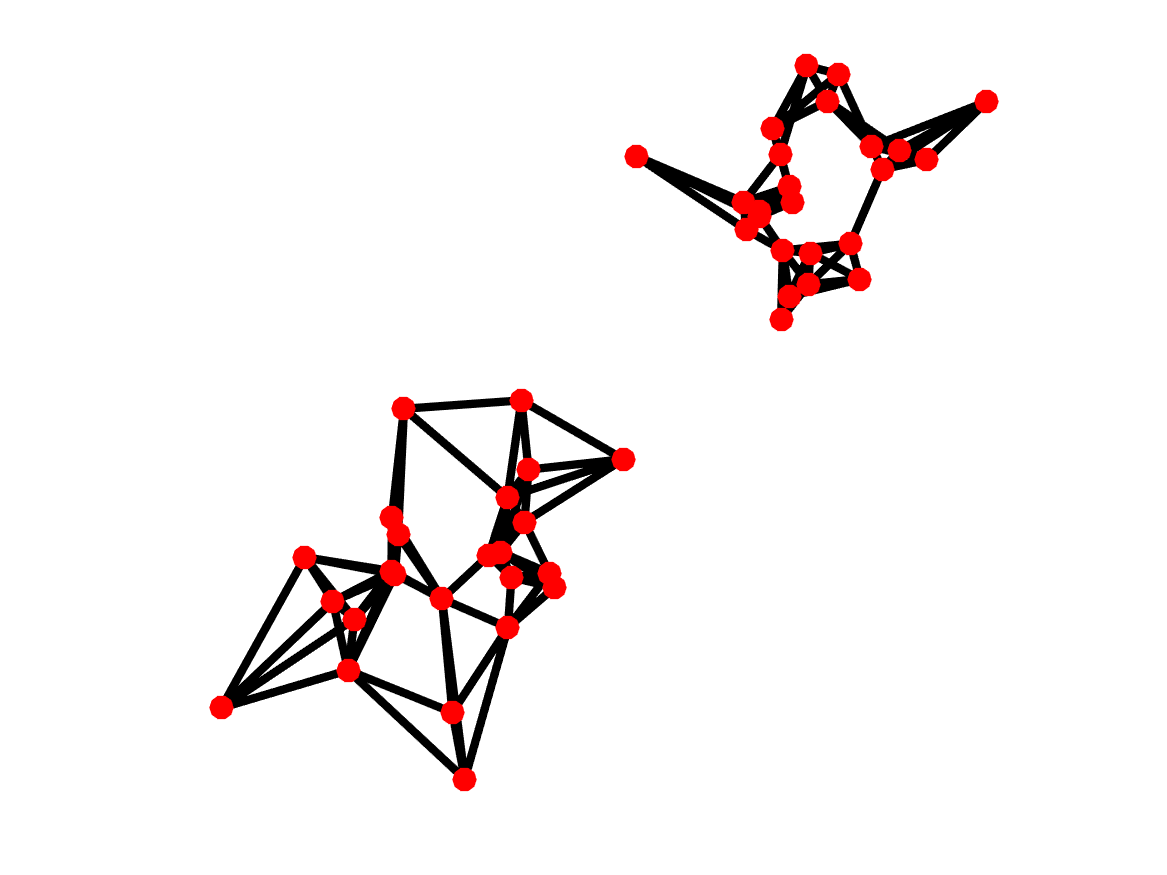
\includegraphics[width=\iwidth,trim=90 0 80 0, clip=true]{eigLap-nnc-2} & 
	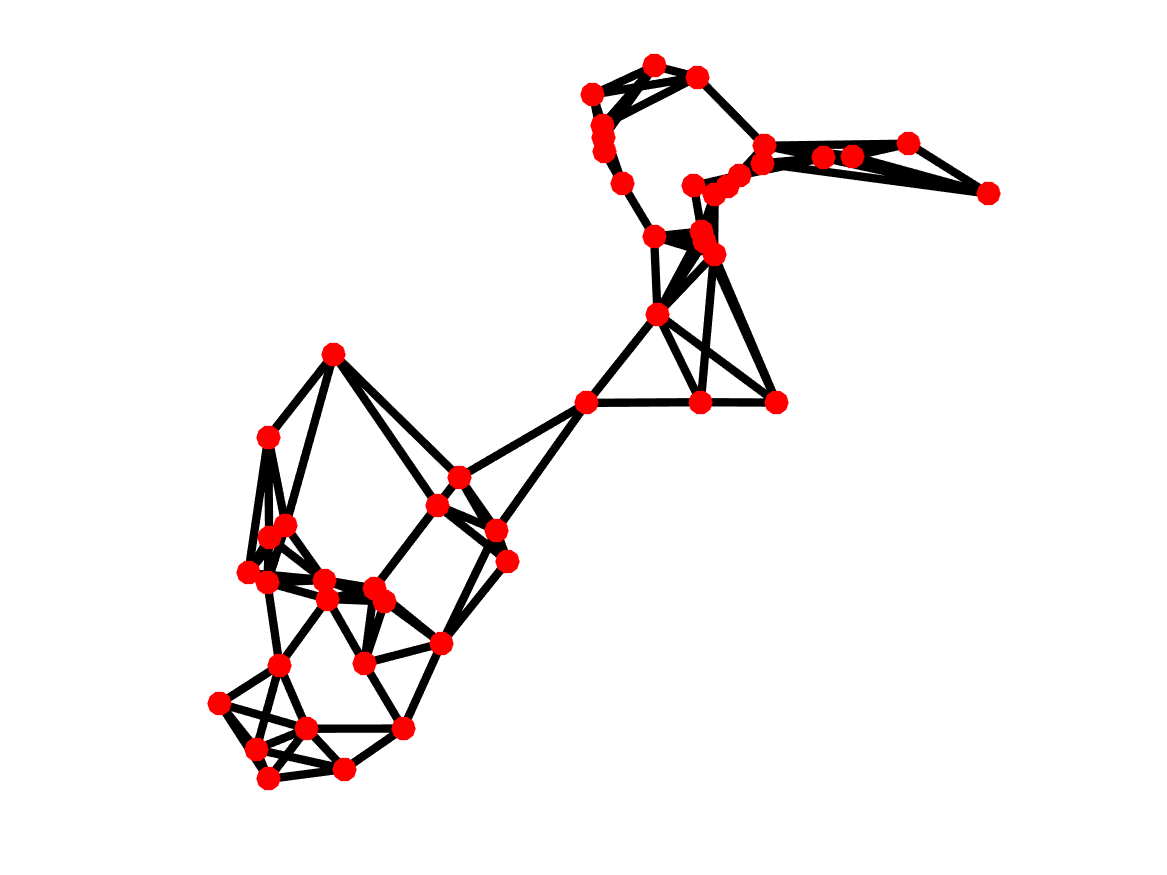
\includegraphics[width=\iwidth,trim=90 0 80 0, clip=true]{eigLap-nnc-1} & 
	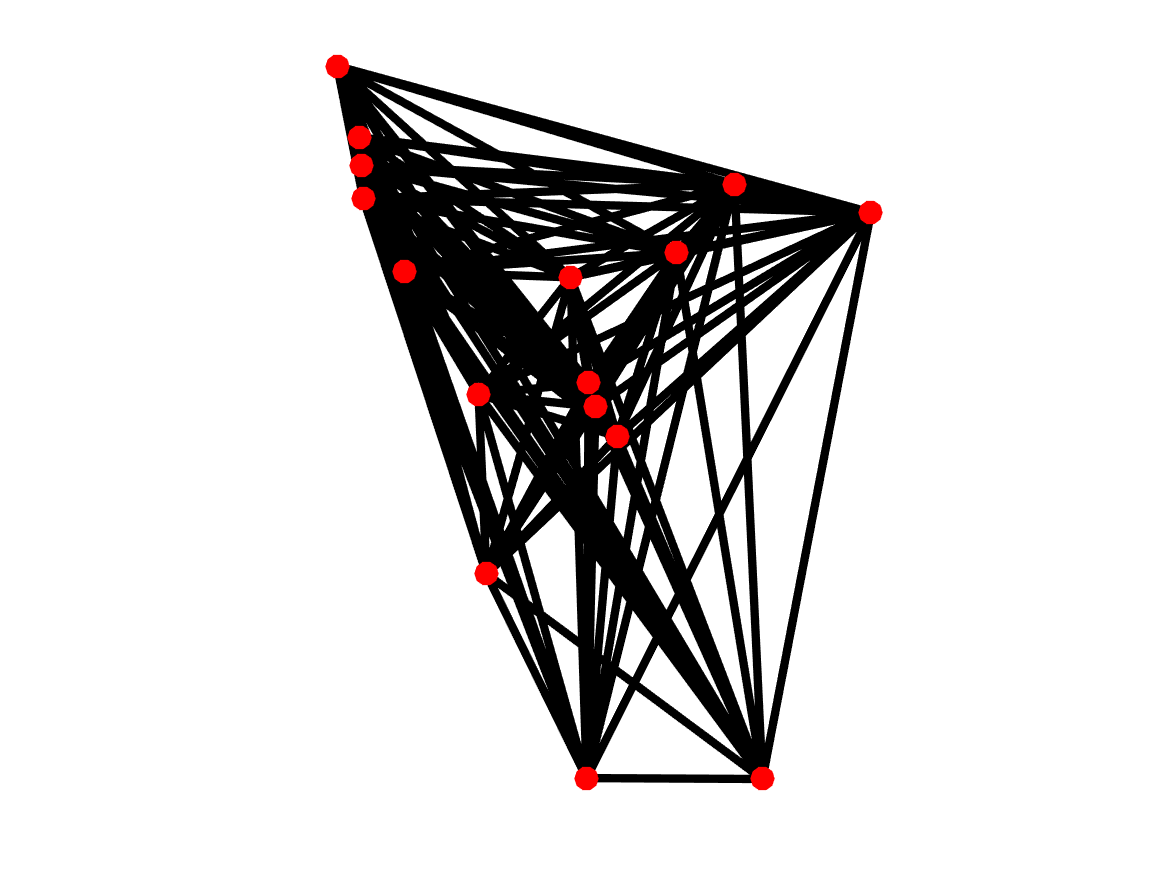
\includegraphics[width=\iwidth,trim=90 0 80 0, clip=true]{eigLap-fc} \\ 
	\scriptsize $\lambda_2 \approx 1.9\cdot 10^{-15}$ &
	\scriptsize $\lambda_2 \approx 8.7\cdot 10^{-3}$ &
	\scriptsize $\lambda_2 \approx 4.0\cdot 10^{-1}$ \\
\end{tabular}
\end{center}
The first (i.e., smallest) eigenvalue is always $0$ with eigenvector $\bfv = [1,\ldots,1]^{\top}$ (why?)

\bigskip

The multiplicity of the eigenvalue $0$ equals the number of connected components in the graph.

\bigskip

The smallest non-zero eigenvalue is the Fiedler eigenvalue.

\end{frame}

\begin{frame}
\frametitle{Fiedler Vector}

	Assume there is only one connected component. Then, the eigenvector associated with the second eigenvalue can be obtained by solving
	
\begin{columns}
	\column{.6\textwidth}
	\begin{eqnarray*}
	\min_{\bfu\not=\gamma\bfe} && \hf \bfu^{\top} \bfL \bfu \\
	\text{subject to} && \|\bfu \| = 1
	\end{eqnarray*}
	Interpretation: Find the non-constant vector with the minimal energy  (i.e., as smooth as possible)


	\bigskip

	
	\column{.4\textwidth}
	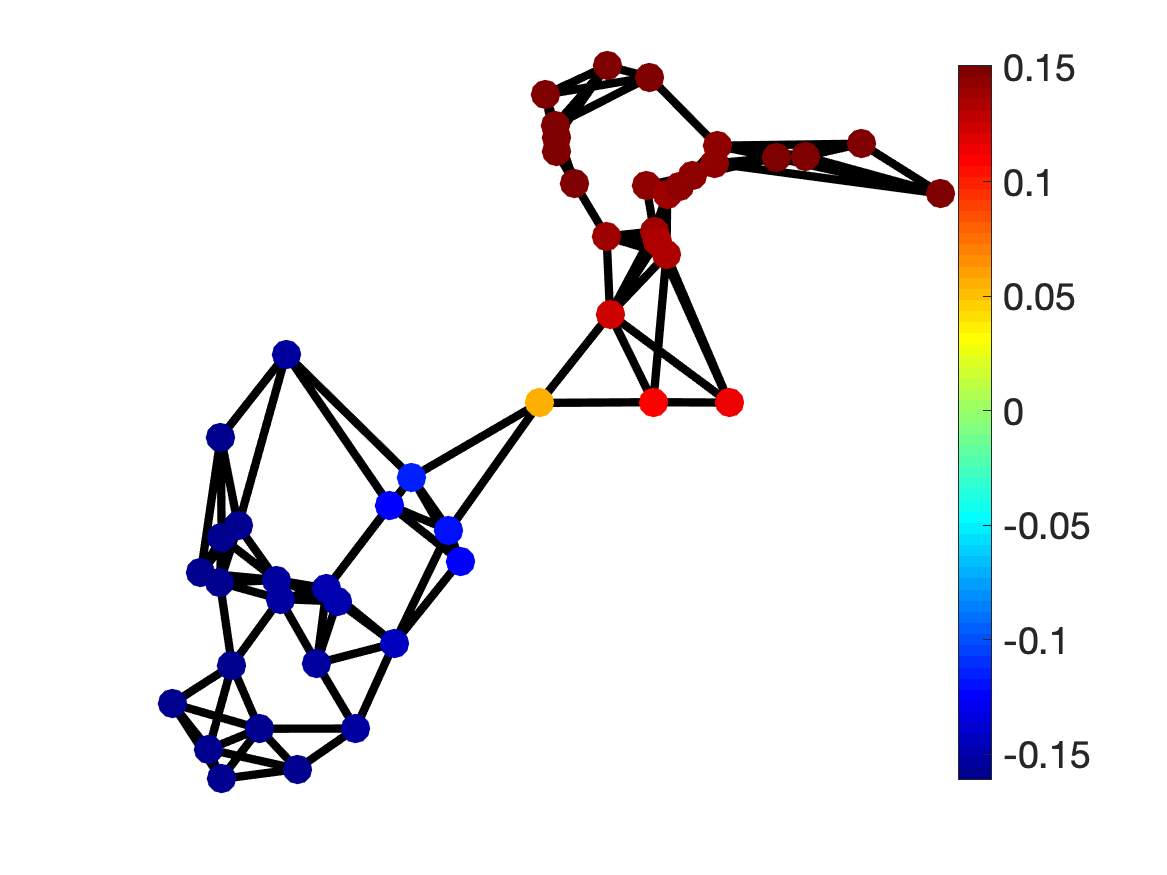
\includegraphics[width=45mm,trim=60 0 30 0, clip=true]{eigLap-nnc-2-fiedler} \\ 
\end{columns}
	It (approximately) holds that $\bfu_i > 0$ for examples in the first group and $\bfu_i<0$ for examples in the second group.



\end{frame}

\begin{frame}
\frametitle{Computing the Fiedler Vector}


The Fiedler vector can be computed by solving the optimization problem
\begin{eqnarray*}
\min_{\bfu\not=\gamma\bfe} && \hf \bfu^{\top} \bfL \bfu \\
\text{subject to} && \|\bfu \| = 1
\end{eqnarray*}


\bigskip

General idea:
\begin{itemize}
\item
For small problems use eig solver of a dense matrix
\item
For large problem use iterative methods - inverse iteration, Krylov methods, randomized linear algebra
\end{itemize}

\bigskip

Simple (but not very efficient) option is the power method:
$$ \bfv_{k} = \bfL^{\dag} \bfu_k \quad \quad \bfu_{k+1} = {\frac {\bfv_k}{\|\bfv_k\|}},\quad k=1,\ldots $$


\end{frame}


% section graph_laplacians (end)


\section{Spectral Clustering Algorithms} % (fold)
\label{sec:spectral_clustering_algorithms}
\begin{frame}
	\frametitle{Algorithm: Normalized Spectral Clustering~\cite{NgEtAl2002}}
	
	Input: Weighted adjacency matrix $\bfW$\\
	Hyperparameters: $n_c$ (no. of clusters), $n_v$ (number of eigenvectors), $k,\sigma$ (for constructing $\bfW$)
	\begin{enumerate}
		\item compute Laplacian $\bfL = \bfD - \bfW$
		\item normalize Laplacian $\bfL_{\rm sym} = \bfD^{-1/2} \bfL \bfD^{-1/2}$ 
		\item compute $\bfu_1,\ldots,\bfu_{n_v}$ the first $n_v$ eigenvectors of $\bfL_{\rm sym}$
		\item define new feature matrix 
		\begin{equation*}
			\bfU = \left( 
				\begin{array}{r}
					\bfu_1^\top\\
					\bfu_2^\top\\
					\vdots\\
					\bfu_{n_c}^\top
				\end{array}
				\right)\in \R^{n_v \times n}
		\end{equation*}
		\item use $k$-means to cluster the columns of $\bfU$ into $n_v$ classes
	\end{enumerate}
	Output: $\bfC \in \R^{n_c \times n}$($\bfC_{ij}=1$ if example $j$ belongs to class $i$)
\end{frame}
% section spectral_clustering_algorithms (end)

\section{Semisupervised Learning} % (fold)
\label{sec:semisupervised_learning}

\begin{frame}
\frametitle{Graph Laplacians in Semisupervised Learning}

Goal: Given $(\bfy_1, \bfc_1), (\bfy_2, \bfc_2), \ldots, (\bfy_k,\bfc_k)$ obtained using
\begin{equation*}
	\bfc = f(\bfy) + \boldsymbol{\epsilon}, \quad \text{($\epsilon$ is  some noise)}
\end{equation*}
estimate $f(\bfy_{k+1}), f(\bfy_{k+2}), \ldots, f(\bfy_n)$. Remarks:

\begin{itemize}
\item
in most cases it is possible to obtain a few labeled data
\item 
can work well if the unlabeled data is similar to the labeled one and $f$ is smooth
\item
typically more robust than unsupervised learning
\end{itemize}

\bigskip

Example : Let $n_c=1$. Solve optimization problem for $\bff \in \R^n$
\begin{equation*}
	\min_{\bff} \hf \sum_{i=1}^k (\bff_i - \bfc_i)^2 + \frac{\alpha}{2} \bff^\top \bfL \bff, \quad \alpha > 0
\end{equation*}


% Assumption: we are given a set ${\cal S}$ where $\bfp_{{\cal S}}^{\rm obs}$ is the probability of each datum to belong to each class
\end{frame}

% \begin{frame}
% \frametitle{Graph Laplacians in Semisupervised Learning}
%
% {\bf Incorporating probabilities - the softmax function}
%
% \begin{itemize}
% \item $\bfp^{\rm obs}$ is a probability, $0 \le \bfp_i^{\rm obs} \le 1$ and $\sum \bfp^{\rm obs} = 1$.®
%
% \item $\bfu$ is unbounded
%
% \item Define $\bfp(\bfu) = {\frac {\exp(\bfu)}{\sum \exp(\bfu)}}$
%
% \item Use cross entropy to compare probabilities, $\bfp(\bfu)$ and $\bfp^{\rm obs}$
% $$ {\ell oss}(\bfu,\bfp^{\rm obs}) = -{\frac 1n} \bfp_{\rm obs}^{\top} \log(\bfp(\bfu)) $$
%
% \end{itemize}
%
% \end{frame}

% \begin{frame}
% \frametitle{From unsupervised to semisupervised learning }
%
% {\bf New goal} - Fit the given labels {\bf and} keep the vector smooth.
%
% $$ \min_{\bfu} \ {\cal E}(\bfu) = {\ell oss}(\bfu,\bfp^{\rm obs}) + {\frac \alpha 2} \bfu^{\top} \bfL \bfu $$
%
% \begin{itemize}
% \item $\alpha$ tradeoff parameter
% \item Can be estimated using cross validation
% \item Solution using inexact Newton's method
% \end{itemize}
%
% \end{frame}
%
%
% \begin{frame}
% \frametitle{From unsupervised to semisupervised learning }
%
% {\bf Example - classifying nonlinear data}
%
% \begin{center}
% 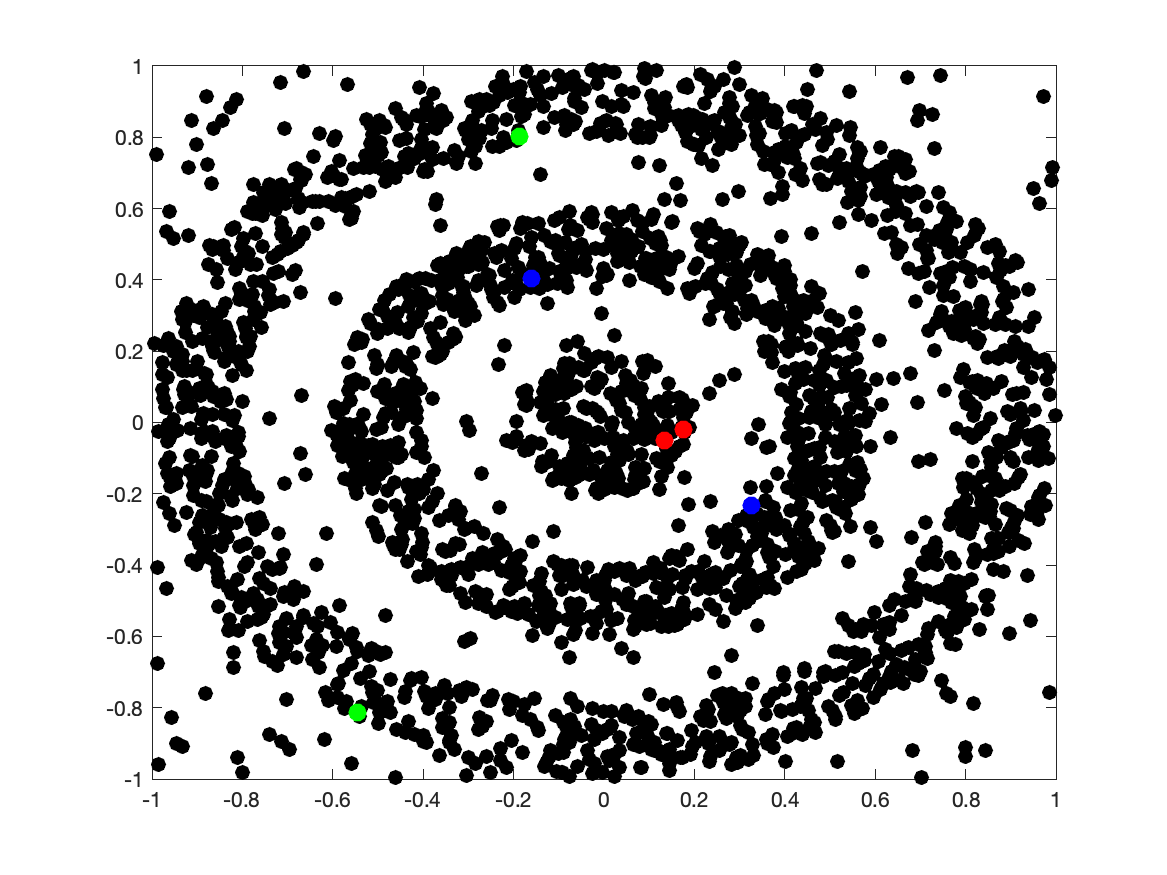
\includegraphics[width=5cm]{dataSemiSup.png}
% \begin{tabular}{cc}
% \includegraphics[width=4.5cm]{graphLapCirc.png} &
% \includegraphics[width=4.5cm]{graphLapCircReord.png} \\
% Graph Lap &   Reordered Graph Lap
% \end{tabular}
% \end{center}
%
%
%
% \end{frame}
%
% \begin{frame}
% \frametitle{From unsupervised to semisupervised learning }
%
%
% \begin{center}
% \begin{tabular}{ccc}
% \includegraphics[width=3.6cm]{probClass1.png} &
% \includegraphics[width=3.6cm]{probClass2.png} &
% \includegraphics[width=3.6cm]{probClass3.png} \\
% Class 1 &  Class 2 & Class 3
% \end{tabular}
% \end{center}
%
%
% \end{frame}


% section semisupervised_learning (end)

\section{Summary} % (fold)
\label{sec:summary}
\begin{frame}
	\frametitle{$\Sigma$: Spectral Clustering for Unsupervised Learning}
	
\begin{itemize}
	\item our focus: graph-based methods
	\item key idea: Given $\bfY$, create weighted undirected graph. Choices:
		\begin{itemize}
			\item distance function (defines similarity)
			\item criteria for edges (control sparsity)
			\item weights for graph (usually based on distance)
		\end{itemize}
	\item spectral clustering requires first few eigenvectors
	\begin{itemize}
		\item naive complexity $n^3$
		\item use iterative/randomized linear algebra for large $n$
	\end{itemize}
	\item semi-supervised learning
	\begin{itemize}
		\item use graph Laplacian to obtain smooth mapping
	\end{itemize}
	\end{itemize}
\end{frame}
% section summary (end)


\begin{frame}[allowframebreaks]
	\frametitle{References}
 \bibliographystyle{abbrv}
\bibliography{NumDNN}

\end{frame}











\end{document}

